\documentclass{article}
\usepackage{graphicx}
\usepackage{hyperref}
\usepackage{float}

\begin{document}

\section{Performance of PKBD Clustering on Real World Datasets}

\subsection*{Introduction}

We have applied the PKBD clustering to the following datasets that reflect variety in terms of sample size, dimensions, and number of clusters. In what follows, we provide a description of the various datasets, describe in detail the preprocessing steps, and provide the results. The associated datasets and scripts can be accessed in the GitHub repository at \url{https://github.com/rmj3197/QuadratiK-Performance}. 

\begin{enumerate}
    \item Birch Dataset II \cite{Birchsets}: This dataset contains $300,000 \times 2$ dimensional synthetic data vectors that represent one of the three patterns shown in Figure \ref{fig:birch}. The dataset can be found at - \url{https://cs.joensuu.fi/sipu/datasets/}. 
    \begin{figure}[H]
    \centering
    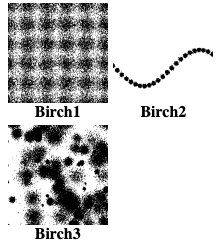
\includegraphics[width=0.25\linewidth]{images/birch_patterns.png}
    \caption{The vectors in the Birch dataset represent one of the three clusters. Image is taken from \url{https://cs.joensuu.fi/sipu/datasets/}.}
    \label{fig:birch}
    \end{figure}

    \item 20 Newsgroups Text Dataset: This dataset is a part of the \texttt{scikit-learn} package \cite{scikit-learn}. This dataset is a collection of approximately 18,000 news posts, partitioned (nearly) evenly across 20 different newsgroups. More information of the dataset can be found at: \url{http://qwone.com/~jason/20Newsgroups/}. 

    \item Reddit Text Dataset: This text dataset is a part of Massive Text Embedding Benchmark (MTEB) \cite{muennighoff-etal-2023-mteb}. This dataset contains titles of Reddit posts from subreddits. For this work, we use the subset of the ``test" set of the data (data split number 13 out of 25) available from \url{https://huggingface.co/datasets/mteb/reddit-clustering}. 

    \item StackExchange Text Dataset: This dataset is also part of the MTEB. This dataset contains titles of questions posted on various StackExchanges. The clustering is performed to identify the different StackExchange communities from which the question titles are collected. In this work, we have used a subset of the ``validation" set (data split number 9 out of 25) of the dataset. The dataset can be found at \url{https://huggingface.co/datasets/mteb/stackexchange-clustering}. 
    
    \item 3 Newsgroups Text Dataset: In this dataset we specifically select three groups from the 20 Newsgroups Text Dataset. The groups selected are: \texttt{omp.os.ms-windows.misc}, \texttt{rec.sport.hockey}, and \texttt{soc.religion.\\christian}, which represent news related to the operating system MS Windows, Hockey, and Christianity. We apply the clustering algorithm just to a subset of the data consisting of these three groups. 

    \item arXiV Text Dataset: This dataset was introduced in \cite{8675939} and is now also part of the MTEB. This dataset was originally curated for classification purposes, where 10,000 words from papers were extracted to train classifiers to predict the paper category among 11 arXiv classes. In our work, we use the ``test" set of the data obtained from \url{https://huggingface.co/datasets/mteb/ArxivClassification}. 

    \item Hand-written Digits Image Dataset: This $8 \times 8$ pixels image dataset is introduced in \cite{kaynak1995methods}. This dataset contains images of handwritten digits from 0-9, representing the 10 classes where each class refers to a digit. This dataset is available in the \texttt{scikit-learn} package and also available on UCI ML Repository at \url{https://archive.ics.uci.edu/dataset/80/optical+recognition+of+handwritten+digits}. Representative images from the various classes are shown in Figure \ref{fig:digits}. 

    \begin{figure}[H]
        \centering
        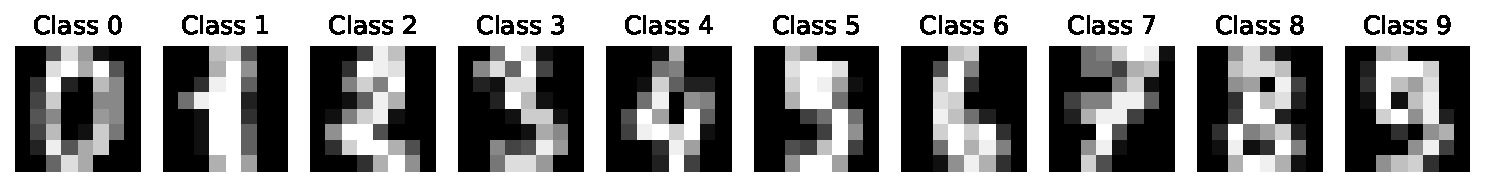
\includegraphics[width=\linewidth]{images/digits_classes.pdf}
        \caption{Example images for each digit from the Hand-written Digits Image Dataset.}
        \label{fig:digits}
    \end{figure}

    \item Detect AI Generated vs Student Generated Text Dataset: This dataset is taken from Kaggle at \url{https://www.kaggle.com/datasets/prajwaldongre/llm-detect-ai-generated-vs-student-generated-text}. The dataset consists of text written by either a student or a large language model (LLM). The goal is to identify the clusters representing the LLM-generated and the student-written text. 

\end{enumerate}

\subsection*{Data Preprocessing}

\begin{figure}[H]
    \centering
    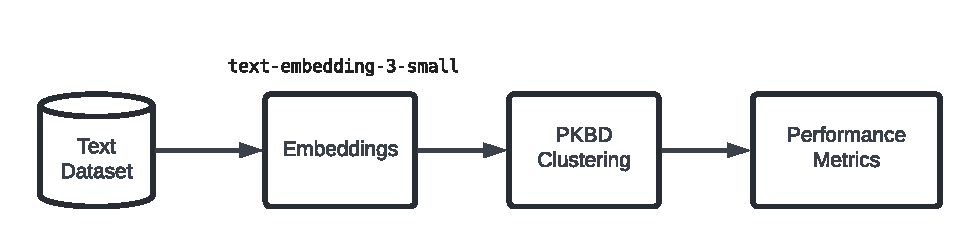
\includegraphics[width=\linewidth]{images/Workflow.pdf}
    \caption{Pipeline used for clustering text datasets.}
    \label{fig:pipeline}
\end{figure}

For clustering text datasets, we have used the workflow depicted in Figure \ref{fig:pipeline}. The text is first converted into embeddings using the \texttt{text-embedding-3-small} embedding model provided by OpenAI. More information on the text embedding model can be found in \cite{Vectorem72:online}. The obtained embeddings are used as the data vector to perform the PKBD clustering. The \texttt{text-embedding-3-small} embedding model used in our work supports a maximum of 8191 tokens. We removed any text containing five or fewer tokens. Additionally, we set a maximum limit of 7000 tokens. If a text exceeded this limit, it was trimmed to fit within the constraint; otherwise, it was kept as is. The tokenization was performed using the \texttt{cl100k\_base} tokenizer in \texttt{tiktoken} \texttt{Python} library. Embeddings of different sizes are used for various datasets shown to demonstrate that the PKBD clustering algorithm can also be applied to high-dimensional data. In the case of the image dataset, the pixel values are flattened, used for clustering. 

\section{References}
\bibliographystyle{plain}  % You can use other styles like 'ieeetr', 'apalike', etc.
\bibliography{references}  % Pointing to the references.bib file

\end{document}